\documentclass{standalone}
\usepackage{tikz}

\begin{document}
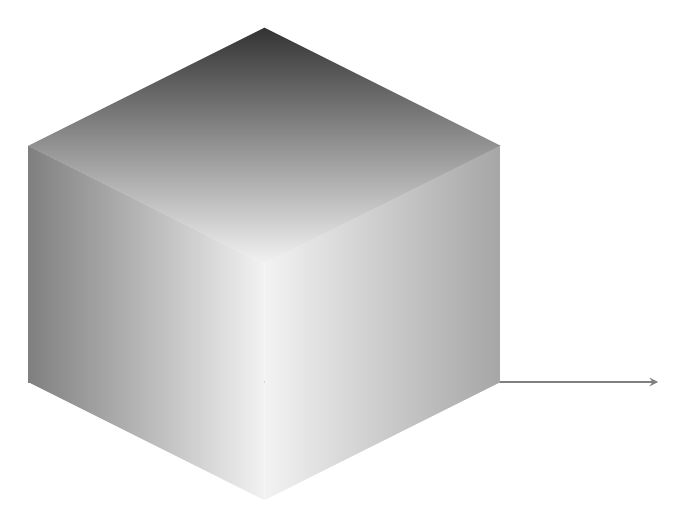
\begin{tikzpicture}

\draw[-stealth,gray] (0,0)--(8,0);

  \shade[yslant=-0.5,right color=gray!10, left color=black!50] (0,0) rectangle +(3,3);
  \shade[yslant=0.5,right color=gray!70,left color=gray!10] (3,-3) rectangle +(3,3);
  \shade[yslant=0.5,xslant=-1,bottom color=gray!10, top color=black!80] (6,3) rectangle +(-3,-3);
\end{tikzpicture}

\end{document}
